\lab{Floating Point Numbers}{Floating Point Numbers}
\label{lab:IEEE}
\objective{Gain a basic understanding of the IEEE floating point standard.}

\section*{Introduction}
Floating point numbers permeate modern computing, but it is not always good to use them without knowledge of what they are and how they work.
A fundamental understanding of the inner workings of floating point numbers can be very helpful when working with a wide variety of floating point computations.
By far the most common floating point standard is the IEEE floating point standard described by in the standards IEEE-754-1985, IEEE-854-1987, and IEEE-754-2008.
These standards outline how floating point numbers are represented in binary form and how operations like addition, subtraction, multiplication, division, and rounding should work.
Most floating point numbers are either 32 or 64 bits long.
32 bit floating point numbers are known as "single precision floating point numbers" and 64 bit floating point numbers are known as "double precision floating point numbers."
There are also 16, 128, and 256 bit versions, but they are much less common.
Floating point numbers in Python are stored as double precision values.
Here we will consider 32 bit floating point numbers.

Before considering any more of the details of IEEE floating point representation, it will be good to establish what a floating point number is at all.
Floating point representation is a way of representing a number that is similar to the "scientific notation" commonly used to represent numbers that are extremely large or small.
In general, a floating point number is a number written in the form $d \times \beta^p$ where $\beta \in \mathbb{N}, \beta \geq 2$ is the base used for computation, $d$ is a decimal (like 1.10110) with base $\beta$ and $p\in \mathbb{Z}$ is the power of $\beta$.
Theoretically, for a given base $\beta \in \mathbb{N}, \beta \geq 2$, any real number $r \in \mathbb{R}$ can be represented at least one way by a series of the form
\begin{equation*}
r = d_0 \beta^{p} + d_1 \beta^{p-1} + \dots = \sum_{i=0}^{\infty} d_i \beta^{p-i}
\end{equation*}
where the $d_i$ are the digits of a decimal number $d$.
This representation is not necessarily unique, but finite approximations of this sort of sum can be useful in performing actual computations.
The floating point representation of a number allows easy representation of real numbers, particularly when they are extremely large, or when they are not integers.
The normal mathematical operations on real numbers apply in the theoretical context.

In real applications, floating point numbers can be used to make an \textit{approximate} representation of \textit{a useful number} of real numbers.
There are uncountably many real numbers, so it is impossible to create a computer system that can distinguish perfectly between all of them, but that is okay since measurements are imperfect and approximate computations are usually good enough.

It is also worth noting that often, for brevity, hexadecimal numbers are used to represent integers and floating point nubmers.
A hexadecimal number is a number base 16.
Each digit of a hexadecimal number can be used to represent four binary digits.
The letters a through f are used to represent the additional 6 values needed.
For example a1f23 is the same as 10100001111100100011.
Python has the built in functions \li{bin} and \li{hex} to convert integers to binary and hexadecimal values.
A binary and hexadecimal numbers stored as strings can be converted to integers using the \li{base} argument of the built in \li{int} funciton.
For example \li{int("a1f23", base=16)} will return 663331, the base 10 representation of the number.

\begin{problem}
\begin{itemize}

\item Make a Python class representing an arbitrary precision floating point number.
This shouldn't be too hard since Python's integers are arbitrary precision as well, just store one integer representing the exponent in some way and another representing the significand.
Make methods to do all of the following:
	\begin{itemize}

	\item Convert a floating point object to a Python float.

	\item Print the floating point number correctly.

	\item Copy the floating point number.

	\item Perform addition of two of your floating point objects (perform all operations without any sort of rounding first).

	\item Perform subtraction of two of your floating point objects.

	\item Perform multiplication of two of your floating point objects.

	\item Truncate the significand of the floating point number to remove all digits below a given power of 10.

	\end{itemize}

\item Now, make another class using the class you just wrote that tracks errors in computation.
Track two values, one for the exact value, and one for the exact error.
Computations involving the value and error should be carried out like they would be for your arbitrary precision floating point class.
Have it track the exact value of the significand and the error until you have it truncate all digits that fall within the error.
Make methods that do all of the following:
	\begin{itemize}

	\item Print the floating point number correctly.

	\item Copy the floating point nubmer.

	\item Perform addition of two of your floating point objects.
		Be sure to add the corresponding errors as well to represent that the possible range of values has increased.

	\item Perform subtraction of two floating point objects.
		Again, be sure to add the corresponding errors.

	\item Perform multiplication of two floating point objects.
		Here's how you can calculate the error term:
		Given two floating point numbers $a\pm\epsilon$ and $b\pm\delta$ where $a$ and $b$ are the values and $\epsilon$ and $\delta$ are the error terms, the result will be $ab \pm a\delta \pm b\epsilon \pm \epsilon\delta$.
		The first term in the expanded product will be the significand of the product and the rest will be the new error term.
		Be sure to take absolute values of $a$ and $b$ when calculating the error so that there is never a negative error term.

	\item Truncate the floating point number to the smallest power of ten that is larger than the error term.
		Set the new error term to be this same power of ten.
		(If you want to do many different calculations involving these floating point numbers, you may, at times have to truncate the values to prevent the integer storing the significand from becoming too large.)

	\end{itemize}

\end{itemize}
\end{problem}

\section*{Binary Representation}
A 32 bit floating point number is represented by 32 bits, each storing either a 0 or a 1.

The first bit in the binary representation of a floating point number represents the sign of the number.
If it is 0, the number is positive.
If it is 1, the number is negative.

The next 8 bits are used to store the exponent of the floating point number.
The exponent does not have an explicit sign bit, but is instead scaled so that the counting runs from -127 to 128.

The final 23 bits are used to store the binary decimal number.
This portion of the number is often called the "mantissa" or the "significand".
Since the first number of any decimal in binary is always one, the first number in the significand is assumed to be one and the bits included in the significand are used to represent the remaining digits.

For example, the following is the binary representation of the number .25.

\begin{equation*}
\underbrace{0}_{sign} \underbrace{01111101}_{exponent}\underbrace{(1.)}_{Implied 1.} \underbrace{00000000000000000000000}_{significand}
\end{equation*}

Since there is a limit on the number of digits used to represent the significand, rounding must occur at each step.
There are several possible rounding conventions, but IEEE floating point rounds the significand to the nearest even value, which in binary means that the last digit must become 0.
For example, using binary decimals, the value $1011011.1$ would round to $1011100$ since that is the nearest even number.

Since rounding occurs after each operation, addition, subtraction, multiplication, and division behave \textit{approximately} how they should.
In some cases, the usual properties you would expect from these operations do not hold.
More on that later.

For a double precision floating point number, there is still one bit to store the sign.
There are 11 bits to store the exponent, and 52 bits used to store the value (with the one still implied).

Floating point operations on modern processors are heavily optimized.
There are built in operations that allow for addition, subtraction, multiplication, division, square roots, and several other operations.
Floating point operations are actually a common way of measuring the performance of computer systems.
What is considered a single floating point operation depends somewhat on the system.
Some processors can perform a single addition and multiplication in a single clock cycle, so a floationg point operation is sometimes considered to be an addition and a multiplication.
It can also be measured as an addition or a multiplication.

The highest and lowest values in the exponent are reserved for modified numbers.
Zero is represented using the smallest exponent value (binary 0, representing a negative power of 2 since the exponent is scaled) with a significand of 0.
When the exponent is as small as possible, the significand is no longer considered normalized and the implied one is no longer considered.
This allows for the representation of even smaller numbers, but it implies the loss of some precision.
For example, the following code in Python yields 0
\begin{lstlisting}
1.123456789012345 * 10.**-306 * 10.**153 * 10.**153 - 1.123456789012345
\end{lstlisting}
While this yields -0.0365123681616.
\begin{lstlisting}
1.123456789012345 * 10.**-322 * 10.**161 * 10.**161 - 1.123456789012345
\end{lstlisting}
Numbers represented in this way are called "denormalized numbers" or "subnormal numbers."
Floating point zero is also still allowed to have a sign, so for example, \li{-0.} is valid in Python and prints as \li{-0.0}.
\li{0.} is considered equal to \li{-0.}, but the sign still carries through in multiplication, so for example \li{-0. *  0.} is \li{-0.}.
There are no analogues of the denormalized numbers.
The values of the highest exponent are used to store different kinds of infinity and "nan" values (nan stands for "not a number").
IEEE floating point allows for both negative and positive infinity.
\li{nan} values are defined to never be equal to one another.
Positive and negative infinity can be used for equality testing, for example, the following returns \li{True}.
\begin{lstlisting}
a = (10.**300)
a *= a # a is now positive infinity
a == a
\end{lstlisting}

% see how they measure it at http://software.intel.com/en-us/articles/estimating-flops-using-event-based-sampling-ebs

\section*{Fast Approximation of the Square Root}
% An amusing application, see http://en.wikipedia.org/wiki/Methods_of_computing_square_roots#Approximations_that_depend_on_IEEE_representation
There are a variety of flaws involved with floating point computations, but those will be discussed in a later lab.
Here we will present an example of a clever manipulation of the IEEE floating point format.
Around the end of the 90's an algorithm was discovered which can give a quick approximation of the square root of a number.
It takes advantage of the layout of the bits in the IEEE floating point standard.
The main idea of it is that the exponent of a binary floating point number $d$ can be used as a rough approximation of the number $\log_2\left(d\right)$.
In performing this computation, we must account for the fact that the exponent has been scaled to allow representation of negative numbers.
The smallest exponent for 32 bit floating point integers is $-2^7 - 1 = -127$.
Since a floating point number has 23 bits in the significand, scaling the exponent can be represented in integer form as addition of $2^{30} - 2^{23}$.
Once we have scaled the exponent, we can divide it by two.
We then scale the exponent back to its original value.
With some extra arithmetic, the two scaling values can be reduced into the addition of a single constant.
When all is said and done, some simple code to calculate the square root of a function looks like this:
\begin{lstlisting}
def pysqrt32(A, reps):
    Ac = A.copy()
    I = Ac.view(dtype=np.int32) # get an integer view of the array
    I >>= 1 # divide by two using a binary bit flip
    I += (1<<29) - (1<<22) # scale by a constant value
    for i in xrange(reps):
        Ac = .5 *(Ac + A / Ac) # use an iterative method to increase accuracy, reps is the number of times.
    return Ac
\end{lstlisting}
The iterative method mentioned here is Newton's method, it is discussed at length in Volume 1, this is one of its many applications.
Without using any additional iterations of Newton's method, the above code gives the approximation to the square root shown in Figure \ref{float:sqrtapprox0}.
With one iteration of Newton's Method, the above code gives the approximation shown in Figure \ref{float:sqrtapprox1}.
Notice that there is no visible difference between the square root and the approximation.
The results should be the same for 64 bit floating point numbers.

\begin{figure}
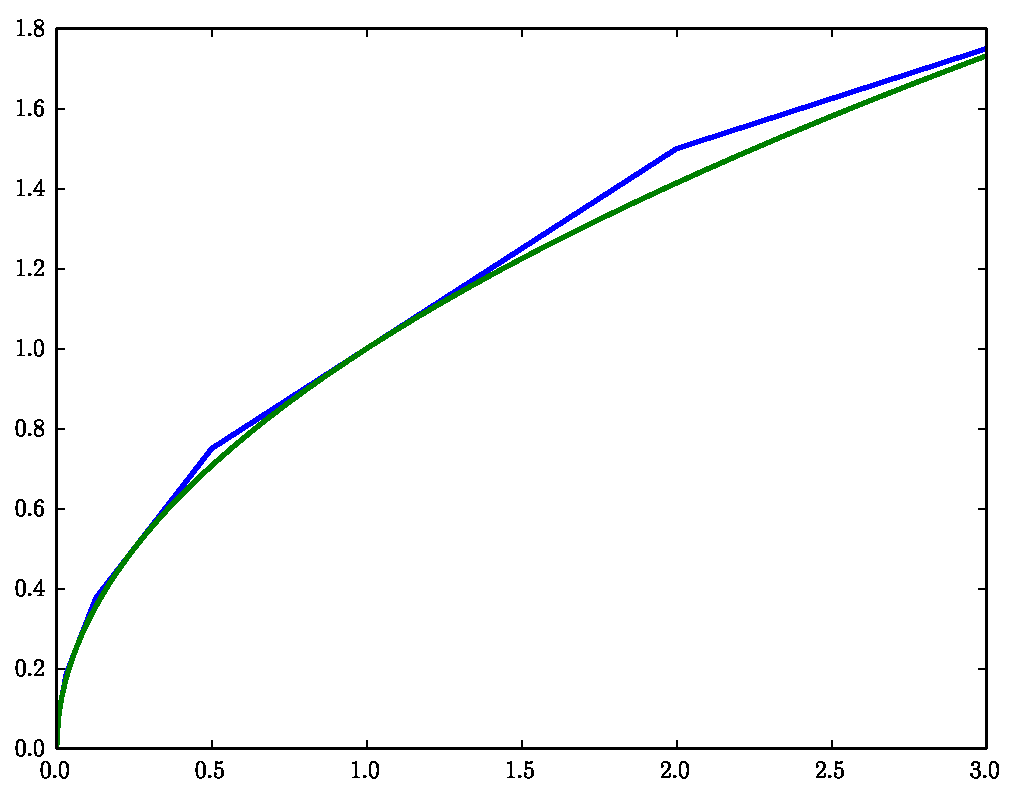
\includegraphics[width=\textwidth]{sqrt0}
\caption{The initial approximation for the square root chosen using the binary representation of the floating point number}
\label{float:sqrtapprox0}
\end{figure}

\begin{figure}
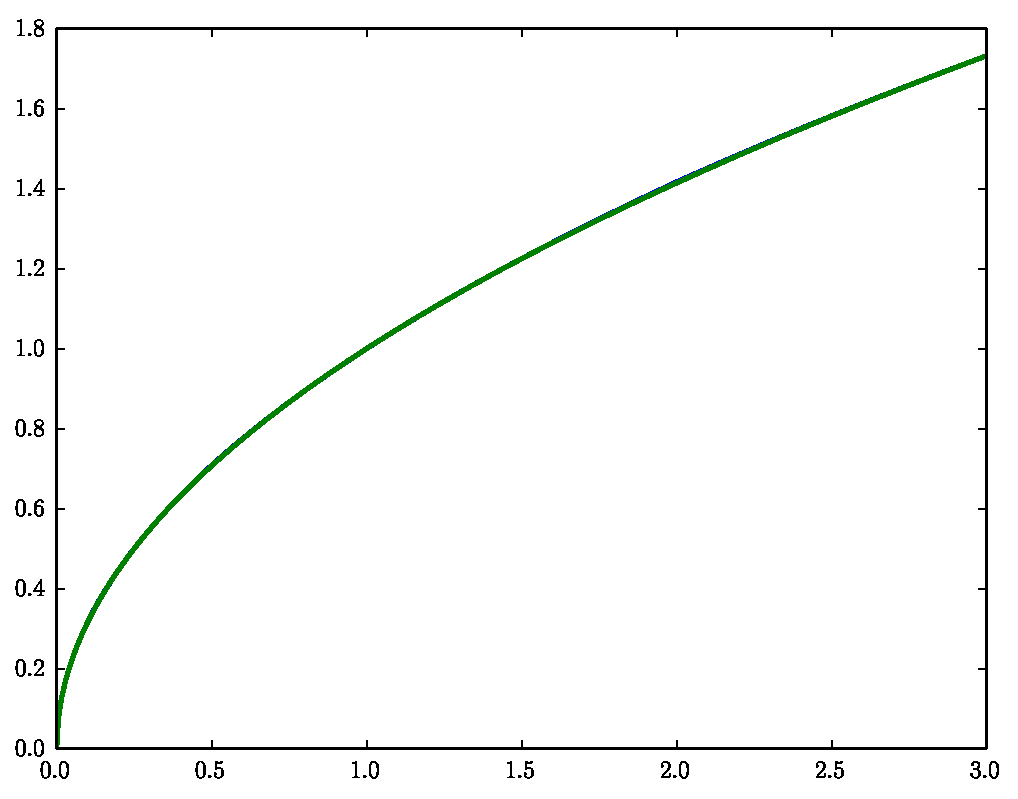
\includegraphics[width=\textwidth]{sqrt1}
\caption{The approximation of the square root after one iteration of an iterative method to increase accuracy.}
\label{float:sqrtapprox1}
\end{figure}

Something similar can be done to find the reciprocal of the square root.
The first two of the following Cython functions calculate the inverse square root for 32 and 64 bit floating point arrays respectively.
The last two functions are equivalents that use the square root function built into C.

\lstinputlisting[name=]{sqrts.pyx}

\begin{figure}
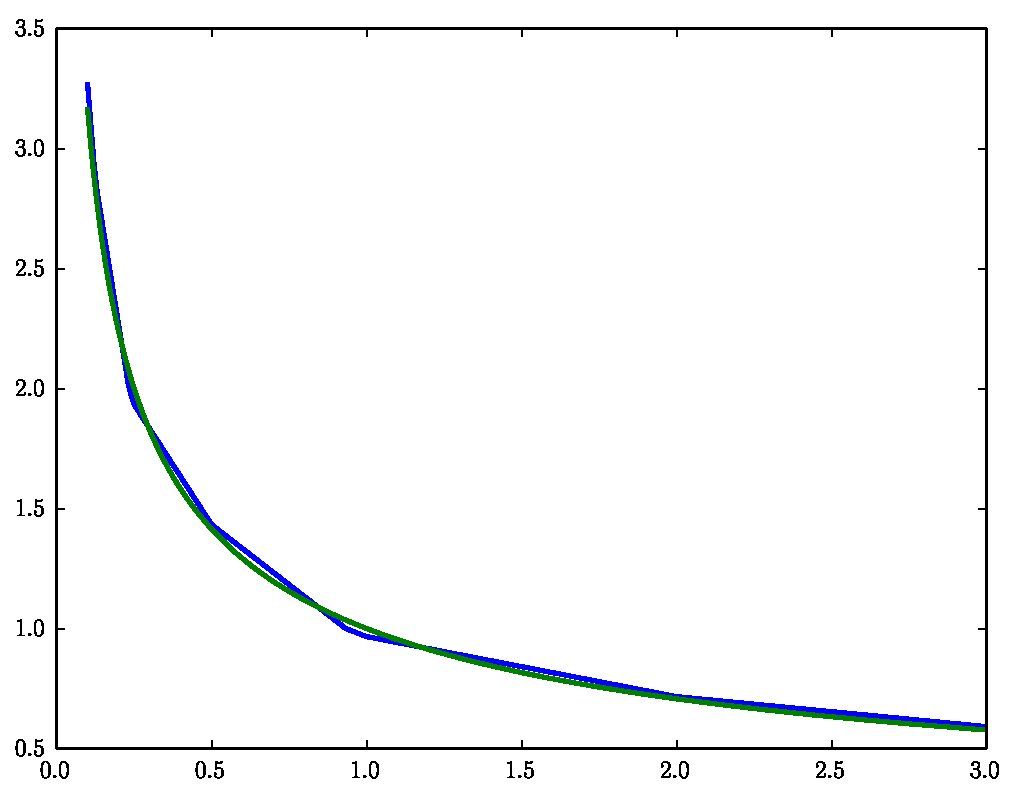
\includegraphics[width=\textwidth]{invsqrt0}
\caption{An initial guess for the inverse square root of a number obtained using the floating point representation.}
\label{float:invsqrt0}
\end{figure}

\begin{figure}
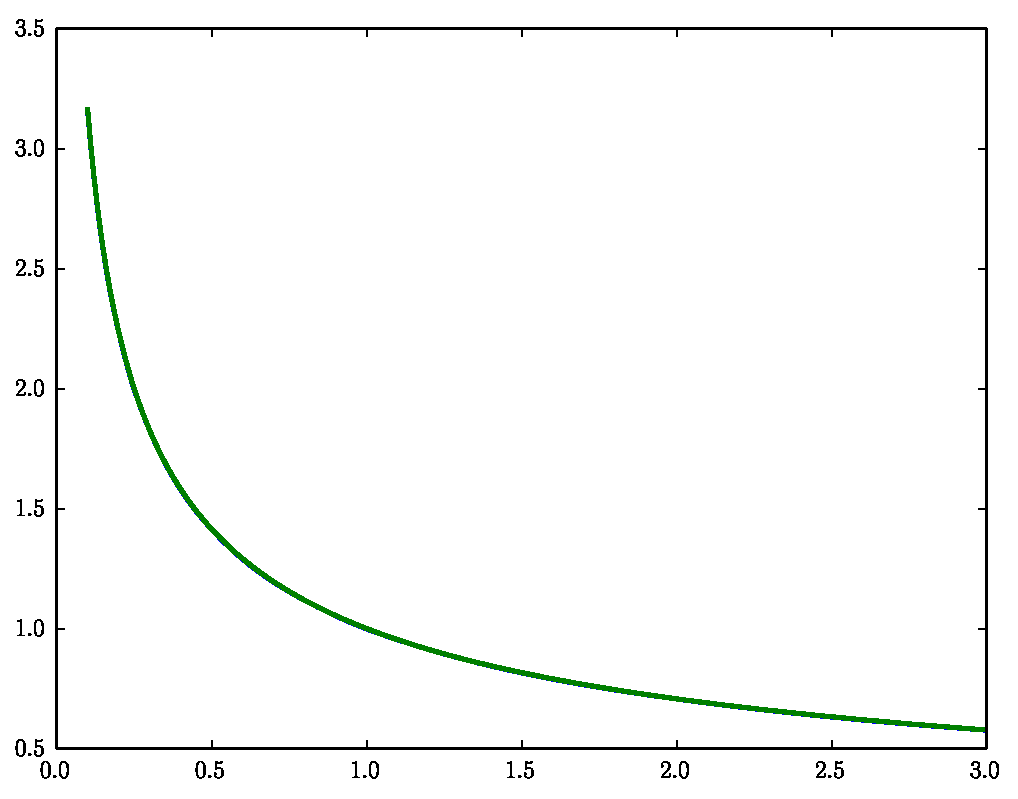
\includegraphics[width=\textwidth]{invsqrt1}
\caption{An approximation for the inverse square root of a number after one iteration of Newton's Method.}
\label{float:invsqrt1}
\end{figure}

This fast inverse square root has been widely used in computer graphics to quickly normalize vectors.
This is a key part of shading 3D surfaces.
It has also been used in a variety of other applications.

\begin{problem}
Make a version of the square root function above that operates on 64 bit floating point arrays.
Hint: you will have to change the type you use for the new view of \li{Ac} and you will have to change the constants $29$ and $22$.
Notice that $29$ is $32-3$ and that $22$ is $29-(e-1)$ where $e$ is the number of bits used for the exponent.

Time the 64 bit square root against NumPy's square root.
NumPy will probably be faster for full accuracy, but the initial guess should run faster than NumPy's square root.
How do the implementations that take advantage of the format of floating point numbers compare with simply taking the reciprocal of the square root of a number using the square root function built in to C?
Why do you think that is?
\end{problem}

Note: It can be interesting to know about these sorts of bitwise operations but, unless you are desperate to optimize an algorithm a little further, it is probably easier and safer to use the built in implementations.